\documentclass[notitlepage, twocolumn]{article}
\usepackage{fullpage}
\usepackage[affil-it]{authblk}
\usepackage{hyperref}
\usepackage{algpseudocode}
\usepackage[]{algorithmicx}
\usepackage{algorithm}
\usepackage{amsfonts}
\usepackage{amsmath}
\usepackage{amssymb}
\usepackage{graphicx}

\def\ft{\mathcal{F}}
\algblockdefx[spawn]{Spawn}{EndSpawn}
[1]{\textbf{spawn process for} #1 \textbf{do}}
{\textbf{end spawn}}

\def\CC{\mathbb{C}}	% Complex

\newcommand{\set}[1]{\lbrace #1 \rbrace}
\newcommand{\paren}[1]{\left( #1 \right)}

\title{\bf
GPU Accelerated Fast Fourier Transform
}

\date{December 2015}
\author{
Matt McCarthy
}
\affil{Christopher Newport University\\
\texttt{\href{mailto:matthew.mccarthy.12@cnu.edu}{matthew.mccarthy.12@cnu.edu}}
}

\begin{document}
\maketitle

\noindent\textbf{Abstract}
We empirically investigate the performance benefits of parallel fast Fourier transform running on the GPU over a sequential version running on the GPU.

\section{Background}

\subsection{Discrete Fourier Transform}

The discrete Fourier transform is a mathematical transformation that takes a set of Complex-valued signals and outputs a set of Complex-valued frequencies.
For an $n$-dimensional Complex-valued vector $\mathbf{X}$, the discrete Fourier transform $\mathbf{Y}=\mathcal{F}(X)$ is given by
\[
	Y_j = \sum_{k=0}^n x_k \omega^{jk}
\]
where $\omega$ is the $n$-th root of unity, $e^{2\pi i/n}$.
Since $\mathbf{Y}$ is an $n$-dimensional, Complex-valued vector, we can see that the discrete Fourier transform has a complexity of $\Theta(n^2)$.

\subsection{Fast Fourier Transform}

Furthermore, we can split the discrete Fourier transform into even and odd sums for $n=2m$, yielding
\[
	Y_j = \sum_{k=0}^m x_{2k}\omega^{2jk} + \omega^j\sum_{k=0}^m x_{2k+1}\omega^{2jk}
\]
which is two seperate discrete Fourier transforms.
Suppose $n=2^k$.
If we iterate this process, we get the following algorithm called the one-dimensional, unordered radix 2, fast Fourier transform.

\begin{algorithmic}[1]
	\Function{R-FFT}{$\mathbf{X}$,$\mathbf{Y}$,$n$,$\omega$}
		\If{$n$=1}
			\State $y_0=x_0$
		\Else
			\State Let $\mathbf{Q}=\mathbf{0},\mathbf{T}=\mathbf{0}\in\CC^n$
			\State Let $\mathbf{X_e}=(x_0, x_2,\ldots,x_{n-2})$
			\State Let $\mathbf{X_o}=(x_1, x_3,\ldots,x_{n-1})$
			\State \Call{R-FFT}{$\mathbf{X_e}$,$\mathbf{Q_e}$,$n/2$,$\omega^2$}
			\State \Call{R-FFT}{$\mathbf{X_o}$,$\mathbf{T_o}$,$n/2$,$\omega^2$}
			\ForAll{$j\in\set{0,1,\ldots,n-1}$}
				\State $y_j=q_{j\mod{n/2}}+\omega^i t_{j\mod{n/2}}$
			\EndFor
		\EndIf
	\EndFunction
\end{algorithmic}

\subsubsection{Cooley Tukey}

Furthermore, we have an iterative formulation of the prior algorithm, called the Cooley Tukey algorithm for one-dimensional, unordered radix 2, fast Fourier transforms.

\begin{algorithmic}[1]
	\Function{I-FFT}{$\mathbf{X}$,$\mathbf{Y}$,$n$}
		\State $t:=\lg n$
		\State $\mathbf{R}=\mathbf{X}$
		\For{$m=0$ to $t-1$}
			\State $\mathbf{S}=\mathbf{R}$
			\For{$l=0$ to $n-1$}
				\State Let $(b_0b_1\ldots b_{t-1})$ be the binary expansion of $l$
				\State $j:=(b_0\ldots b_{m-1}0b_{m+1}\ldots b_{t-1})$
				\State $k:=(b_0\ldots b_{m-1}1b_{m+1}\ldots b_{t-1})$
				\State $r_i:= s_j+s_k\omega^{(b_mb_{m-1}\ldots b_0 0\ldots0)}$
			\EndFor
		\EndFor
		\State $\mathbf{Y}:=\mathbf{R}$
	\EndFunction
\end{algorithmic}

From this pseudo-code, we can determine the complexity of fast Fourier transform.
We begin by noting that we iterate through the outer loop precisely $\lg n$ times and the inner loop $n$ times.
Therefore our complexity is $T_1=\Theta(n\lg n)$.

\subsection{Parallelization}

For our parallelization, we use a simplified version of the binary exchange algorithm, a parallelization of the Cooley Tukey algorithm designed for use on a hypercube.
Since our implementation runs on a single GPU, any thread can access any memory location via a pointer.
However, this also complicates the matter by introducing a potential for data races.
We solve this by modifying the algorithm to work as follows.

\begin{algorithmic}[1]
	\Function{PAR-FFT}{$\mathbf{X}$,$\mathbf{Y}$,$n$}
		\State $t:=\lg n$, $BLK:=n/p$
		\State $\mathbf{R}=\mathbf{X}$
		\State $\mathbf{S}=\mathbf{0}$
		\For{$m=0$ to $t-1$}
			\State Swap pointers $\mathbf{R}$ and $\mathbf{S}$
			\Spawn{$l=0$ to $BLK-1$}
				\For{$c=l\cdot BLK$, to $l\cdot(BLK+1)$}
					\State Let $(b_0b_1\ldots b_{t-1})$ be the binary expansion of $c$
					\State $j:=(b_0\ldots b_{m-1}0b_{m+1}\ldots b_{t-1})$
					\State $k:=(b_0\ldots b_{m-1}1b_{m+1}\ldots b_{t-1})$
					\State $r_i:= s_j+s_k\omega^{(b_mb_{m-1}\ldots b_0 0\ldots0)}$
				\EndFor
			\EndSpawn
			\State \textbf{sync}
		\EndFor
		\State $\mathbf{Y}:=\mathbf{R}$
	\EndFunction
\end{algorithmic}
In each iteration, we only write to $\mathbf{R}$ and only read from $\mathbf{S}$.
Since we wait until each thread is complete before moving on to the next iteration, we avoid the potential to use old or incorrect data.

If we inspect the parallelization, we see that the outer loop runs $\lg n$ times.
However, the inner loop is ran on $p$ processes, each of which handle $n/p$ iterations.
Therefore, the computation cost is $\Theta(n/p\lg n)$.
Moreover, for communication we simply do two reads from VRAM on each iteration of the inner loop, however some values will be in cache so we may get better performance than that.
Ergo, the communication cost is $O(n/p\lg n)$.
Thus, the parallel runtime will be $T_p = O(n/p \lg n)$ and is cost optimal if and only if $p\leq n$.

\section{Experimental Design}

The goal of the experiment is to empirically determine the effect of parallelization on the runtime of the Cooley Tukey algorithm.
To this end we want to measure the runtime of fast Fourier transform using differing sizes of $n$, the dimension of our Complex valued vector, and $t$, the number of threads.
Let $\mathcal{N}$ be the set of vector dimensions we will test and let $\mathcal{T}$ be the set of thread counts we will test.
Furthermore, we specify that each $n\in\mathcal{N}$ and each $t\in\mathcal{T}$ be powers of two.

For $t=1$, we will run the Cooley Tukey algorithm on random Complex valued vectors of dimension $n$ for each $n\in\mathcal{N}$.
Otherwise, we run our parallelization of the Cooley Tukey algorithm on Complex valued vectors of dimension $n$ for each $n\in\mathcal{N}$.
Moreover, before and after each run, we copy the input to the GPU and the output from the GPU.
We do not check the output for correctness during the test in order to save time, but instead checked the correctness of the algorithm beforehand.

\section{Test Environment}

\subsection{Test System}

The machine used to run the test has an Intel i7 4770k running at 4.2GHz, 16GB of RAM, and a Nvidia GTX 970 with a core clock of 1342MHz and memory clock of 7000MHz.
The computer was running Arch Linux on Linux kernel 4.2.5 with Nvidia driver version 358.16 and CUDA 7.5.

\subsection{Test Program}

Firstly, all code can be located at \url{https://github.com/matt-mccarthy/fast-fourier-transform} in the \verb|fast-fourier| folder.
We also include a version of the code in the Appendix.

All code was compiled with the CUDA toolkit 7.5 and GCC 5.2.0 with the command \verb|nvcc| \verb| -std=c++11| \verb|-rdc=true| \verb|-arch=compute_52| \verb|-code=sm_52 -O3|.
The library source file is \verb|src/fast-fourier.cu|, and the sequential and parallel main functions are located in \verb|sequential-fft.cu| and \verb|parallel-fft.cu| respectively.

In both the sequential fast Fourier and parallel fast Fourier, we ran into issues with dynamically allocating memory in a CUDA kernel.
Namely, if we allocated and freed often enough, we ran out of memory.
To avoid this issue entirely, we made all allocations of giant arrays occur in main once and then reused those arrays.
As a note, the \verb|binary_stor| array is where we store the binary representation of our index $l$ for each thread.
While this design is suboptimal (ideally, each thread would create its own so others can not touch it), it works and the performance impact should be neglible for large enough $n$.

\section{Results}

\begin{figure}[h!]\label{results}
	\centering

	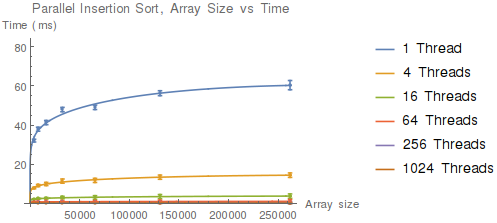
\includegraphics[scale=0.5]{results.png}
	\caption{Runtime vs Array Size}
\end{figure}

\begin{figure}[h!]\label{res-table}
	\centering
	\begin{small}
	\[
		\begin{array}{r|c|c|c|c|c|c|c}
			& 2^{12} & 2^{13} & 2^{14} & 2^{15} & 2^{16} & 2^{17} & 2^{18}\\\hline
			2^0& 32.02 & 37.86 & 41.27 & 47.92 & 49.06 & 56.29 & 60.42\\\hline
			2^2& 7.73 & 9.01 & 9.82 & 11.31  & 11.65 & 13.31 & 14.35\\\hline
			2^4& 2.05 & 2.33 & 2.51 & 2.88 & 2.96 & 3.38 & 3.64\\\hline
			2^6& 0.56 & 0.65 & 0.67 & 0.75 & 0.76 & 0.87 & 0.93\\\hline
			2^8& 0.20 & 0.19 & 0.20 & 0.21 & 0.21 & 0.24 & 0.25\\\hline
			2^{10}& 0.11 & 0.08 & 0.07 & 0.07 & 0.07 & 0.07 & 0.08
		\end{array}
	\]
	\end{small}
	\caption{The table of runtimes generated at $(n,t)$ in ms}
\end{figure}

\autoref{res-table} lists the runtimes for each $t$ (row index) at size $n$ (column index).
Note, however that for $t\geq 2^8$, our standard deviation sometimes exceeded the average, although, our standard deviations up to $t=2^6$ were small enough for us to gain some data.

\subsection{Linear Speedup}

By inspection, we see that $T_{2k}\approx T_{2k+2}/4$, which is exactly what we are looking for. So naively, we can say that this has a linear speedup.
We attempted to find statistical evidence for this by showing that the 

\section{Conclusion}

\section*{Appendix}

\end{document}
